Theorem~\ref{thm:general} says the achievable worst-task excess is bounded
below by $B^2(1 - \deff/(Tr))$, and that this floor is zero exactly when
the $T$ task subspaces are in general position. This section shows that
real LoRA cohorts occupy both regimes, that which one they occupy is
decided by how they were initialised rather than by anything about the
tasks, and that the regime can be read off the adapter weights alone.

\subsection{Why shared initialisation collapses the task subspaces}
\label{subsec:mechanism}

In the reference LoRA implementation~\citep{hu2022lora} an adapter is
$\Delta W = BA$ with $A \in \R^{r \times k}$ drawn from a random
initialisation and $B \in \R^{m \times r}$ initialised to zero. Two
consequences matter here. First, because $B = 0$ at the start, the
gradient with respect to $A$ is proportional to $B$ and therefore vanishes
at initialisation, so $A$ moves comparatively little over training.
Second, in most training pipelines the initialisation is drawn from a
single global seed. If the $T$ adapters of a cohort are trained with that
same seed, as is the natural thing to do when the seed is meant to control
run-to-run reproducibility, then all $T$ adapters begin from an
\emph{identical} $A$ and never move far from it.

The row space of $\Delta W_t = B_t A_t$ is contained in the row space of
$A_t$. If every $A_t$ is a small perturbation of one shared matrix, the
$T$ task subspaces are near-collinear, $\deff$ collapses toward $r$ rather
than $Tr$, and the floor rises toward $B^2(1 - 1/T)$. This is not a
statement about the tasks being similar. It is an artifact of the
initialisation, and it survives even when the tasks are entirely unrelated.

\subsection{Measurement}
\label{subsec:measurement}

We train $T = 4$ adapters at rank $r = 16$ on four base models, giving
$Tr = 64$, for four unrelated tasks (instruction following, code, mathematical
reasoning, and summarisation; full configuration in
Appendix~\ref{app:manifest}). We do this in two conditions. The
\emph{shared} condition uses one global seed for the whole cohort, which
is what our own earlier draft and, as far as we can tell from released
code, much of the merging literature does. The \emph{independent}
condition draws a separate initialisation per task. We repeat the
independent condition three times with different draws, giving cohorts
\texttt{indep1}, \texttt{indep2} and \texttt{indep3}, so that the
comparison is not resting on a single lucky sample.

For each cohort we compute, per layer and then averaged over eight sampled
layers: the median principal cosine between the $T$ task row spaces; the
relative distance $\|\Delta A\|/\|A\|$ between task $A$ factors; the top
singular value $\sigma_{\max}$ of the stacked projectors, which equals
$\sqrt{T}$ under exact collinearity and approaches $1$ under
orthogonality; the soft effective dimension; and the resulting floor.

\begin{table}[t]
\centering
\small
\caption{Subspace geometry, four base models, $T=4$, $r=16$, $Tr=64$.
The three independently initialised cohorts agree to three decimals, so
only \texttt{indep1} is shown per base; \texttt{indep2} and
\texttt{indep3} are in Appendix~\ref{app:geometry}. Floor is
$1 - \deff/(Tr)$, in units of $B^2$.}
\label{tab:geometry}
\begin{tabular}{llccccc}
\toprule
base & init & med.\ cosine & $\|\Delta A\|/\|A\|$ & $\sigma_{\max}$ &
soft $\deff$ & floor$/B^2$ \\
\midrule
Llama-3.1-8B  & shared      & 0.9948 & 0.168 & 1.999 & 16.33 & 0.745 \\
              & independent & 0.0473 & 1.415 & 1.107 & 63.23 & 0.012 \\
\addlinespace
Mistral-7B    & shared      & 0.9947 & 0.159 & 1.999 & 16.28 & 0.746 \\
              & independent & 0.0468 & 1.412 & 1.106 & 63.24 & 0.012 \\
\addlinespace
Qwen2.5-7B    & shared      & 0.9964 & 0.191 & 1.999 & 16.35 & 0.744 \\
              & independent & 0.0500 & 1.412 & 1.131 & 63.08 & 0.014 \\
\addlinespace
Yi-1.5-9B     & shared      & 0.9973 & 0.163 & 2.000 & 16.28 & 0.746 \\
              & independent & 0.0467 & 1.412 & 1.102 & 63.25 & 0.012 \\
\bottomrule
\end{tabular}
\end{table}

\begin{figure}[t]
\centering
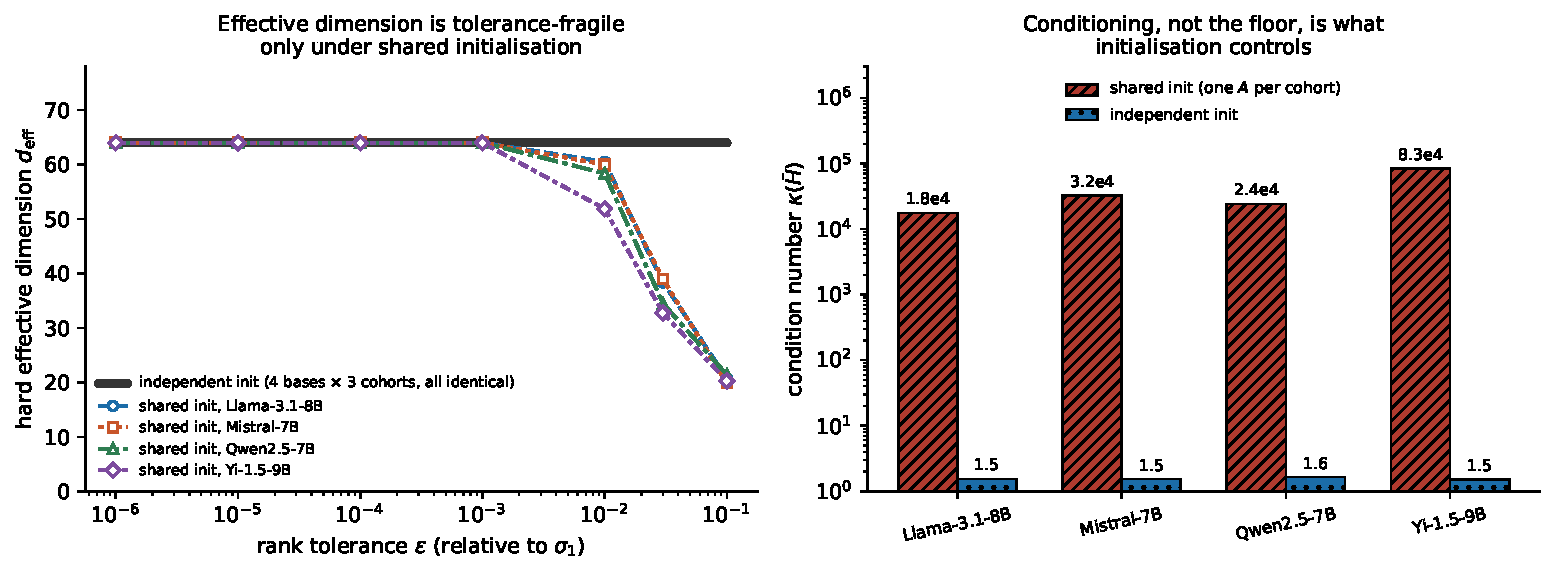
\includegraphics[width=\textwidth]{figures/figure_two_regimes.pdf}
\caption{The two regimes. \textbf{Left:} hard effective dimension against
rank tolerance $\epsilon$. All twelve independently initialised cells
(four bases $\times$ three cohorts) hold $\deff = Tr = 64$ at every
tolerance across four decades; the shared-initialisation cohorts match
only at numerically loose tolerances and collapse to $20.8$ by
$\epsilon = 10^{-1}$. \textbf{Right:} the resulting irreducible floor,
$0.745B^2$ under shared initialisation against $0.012B^2$ under
independent initialisation.}
\label{fig:two-regimes}
\end{figure}

\subsection{Result}
\label{subsec:regime-result}

Table~\ref{tab:geometry} and Figure~\ref{fig:two-regimes} give the
outcome, and the separation is not marginal. Under shared initialisation
the median principal cosine is $0.995$ or above, meaning the task
subspaces are nearly the same subspace; $\sigma_{\max}$ is $1.999$ against
a collinear maximum of $\sqrt{T} = 2$; the $A$ factors have moved
$16$ to $19\%$ from their common start; soft $\deff$ is $16.3$ of $64$,
close to the fully collinear value $r = 16$; and the floor is $0.745B^2$,
essentially the fully collinear $B^2(1 - 1/T) = 0.75B^2$.

Under independent initialisation the same cohort design gives cosines
around $0.047$, $\sigma_{\max}$ near $1.1$, $\|\Delta A\|/\|A\|$ of
$1.41 \approx \sqrt{2}$, which is exactly the value for two independent
vectors of equal norm, soft $\deff$ of $63.2$ of $64$, and a floor of
$0.012B^2$. The floor moves by a factor of $52$ to $64$ depending on the
base.

The hard-tolerance sweep in the left panel of Figure~\ref{fig:two-regimes}
is the sharper statement. Effective dimension computed with a hard rank
tolerance is only meaningful if it is stable in that tolerance. For the
independent cohorts it is completely stable: every one of the twelve
cells returns $\deff = 64$ at every $\epsilon$ from $10^{-6}$ to
$10^{-1}$. For the shared cohort it is not: $\deff = 64$ holds only for
$\epsilon \leq 10^{-3}$, and by $\epsilon = 10^{-1}$ it has fallen to
$20.8$. A shared-initialisation cohort can therefore be made to look
full-dimensional by choosing a permissive tolerance, which is a trap worth
flagging, since $\deff = Tr$ at a loose numerical threshold is exactly
what one would report by default.

\paragraph{Replication.} The three independent cohorts were drawn
separately and agree to three decimal places on every column of
Table~\ref{tab:geometry}. The consistency assertion is enforced in the
figure-generating code rather than checked by eye. Whatever this effect
is, it is not sampling noise.

\subsection{The audit}
\label{subsec:audit}

Everything above is computed from the adapter weight matrices. No forward
passes, no evaluation data, and no merging is involved, so the whole
measurement takes about one CPU minute for a cohort of four rank-16
adapters. We package it as an audit that answers one question before any
merging is attempted: is the cohort in the floor-zero regime, where the
observed merging loss is recoverable slack, or in the floor-positive
regime, where most of it is not.

The practical recommendation follows directly and is uncomfortable for
anyone benchmarking merging methods. If a cohort reports median principal
cosine near $1$ and soft $\deff$ near $r$, then a large part of whatever
worst-task excess is measured on it is irreducible, no merging method can
remove it, and differences between methods on that cohort are being
measured against a floor rather than against zero. The fix is on the
training side and costs nothing: draw the LoRA initialisation
independently per task.

We are careful about how far to push this. We can show that our own
earlier cohorts were degenerate in exactly this way, and we can show what
it does to the floor. We attempted to establish the stronger claim, that
published merging comparisons are confounded by the same effect, and a
pre-registered control we designed for the purpose did not support it. We
withdraw that claim in \S\ref{subsec:withdrawn}.
